\chapter{METODOLOGIA}

A metodologia (Observada na \ref{fig:Fluxograma}) é dividida em 2 partes. Na primeira parte, será utilizada uma simulação no gazebo simulator. A simulação possuirá um ambiente para testar o desempenho de um robô turtlebot. Ocorrerão dois testes, no primeiro teste o robô utilizará apenas ROS 2 enquanto no segundo teste o robô utilizará ROS 2 e Docker. Após a análise[EXPLICAR COMO É FEITA A ANÁLISE] do desempenho nos testes, os dados serão armazenados, analisados e finalmente comparados.
Na segunda parte, ao invés de uma simulação, será utilizado um robô turtlebot real. Os testes são semelhantes aos aplicados na primeira parte, onde o primeiro teste será realizado apenas com ROS 2 enquanto o segundo será realizado com ROS 2 e Docker juntos, para que assim os dados de desempenho possam ser coletados, analisados e então comparados.
As arenas que serão utilizadas na simulação serão baseadas em possíveis arenas que serão montadas na FEI na sala k404. A mesma possui uma arena que pode ser montada e um robô TurtleBot 3 Burger para a realização dos testes, assim será desenvolvida uma simulação com uma arena baseada na arena existente na instituição. A arena possui um caminho, mas o mesmo pode [COLOCAR UMA IMAGEM DA ARENA DA K404] ser alterado com algumas placas que funcionam como paredes, essas paredes permitem a criação de um caminho diferente para o robô podendo ser feito um labirinto, assim seria desenvolvida uma simulação com a mesma ideia para que se pudesse obter dados com uma relação maior. Com relação à parte física, seriam utilizados tanto o robô quanto a arena física para que pudessem ser executados os testes necessários para se adquirir os dados para então analisá-los e compararmos.

\begin{figure}[htb]
    \centering
    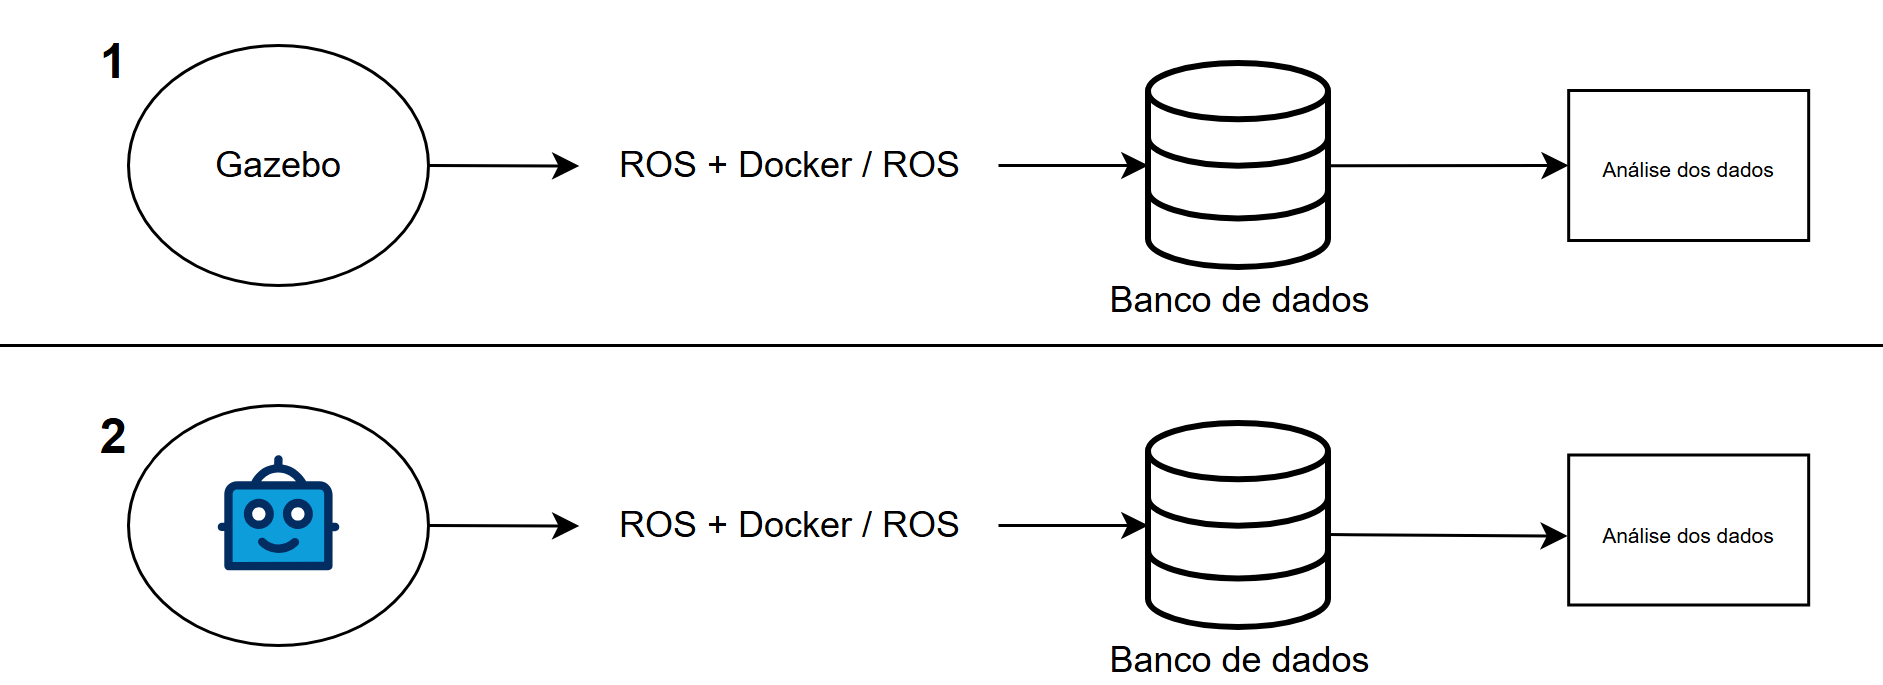
\includegraphics[width=0.9\linewidth]{Figures/FluxogramaTCC.png}
    \caption{Fluxograma do projeto[NECESSITA SER REFERENCIADO]}
    \label{fig:Fluxograma}
\end{figure}